\usepackage{amsmath,amssymb,bm}
\usepackage{braket}
\usepackage{tikz}
\usetikzlibrary{arrows.meta,positioning}


\begin{document}
\subsection{Quantum control in quantum computing}
\label{subsec:quantum_control_qc}

Quantum computation is often introduced in the abstract language of qubits, unitary gates, and quantum circuits. In practice, however, every quantum algorithm must ultimately be implemented through the controlled dynamical evolution of a physical system. The central task of quantum control is therefore to determine a set of experimentally realizable control fields that drive a quantum device from an initial state or propagator to a desired target operation \cite{nielsen2010quantum,dalessandro2007introduction,niu2018ufo}. In a generic closed-system description, the system Hamiltonian can be decomposed into a drift term, which describes the uncontrolled internal dynamics of the device, and a set of control Hamiltonians weighted by time-dependent amplitudes:
\begin{equation}
H(t)=H_{0}+\sum_{k=1}^{m} u_{k}(t)\,H_{k},
\label{eq:control_hamiltonian}
\end{equation}
where $H_{0}$ is the drift Hamiltonian, $\{H_{k}\}_{k=1}^{m}$ are experimentally addressable control generators, and $\{u_{k}(t)\}$ are the corresponding control waveforms. The quantum state $\ket{\psi(t)}$ then evolves according to the time-dependent Schr\"odinger equation
\begin{equation}
i\hbar \frac{d}{dt}\ket{\psi(t)} = H(t)\ket{\psi(t)},
\label{eq:schrodinger_control}
\end{equation}
while the associated propagator $U(t)$ satisfies
\begin{equation}
i\hbar \frac{d}{dt}U(t)=H(t)U(t),
\qquad
U(0)=\mathbb{I}.
\label{eq:propagator_equation}
\end{equation}
Formally, the unitary evolution generated over a control duration $T$ is
\begin{equation}
U(T)=\mathcal{T}\exp\!\left[-\frac{i}{\hbar}\int_{0}^{T} H(t)\,dt\right],
\label{eq:time_ordered_propagator}
\end{equation}
where $\mathcal{T}$ denotes the time-ordering operator. In the context of gate synthesis, the control problem consists of designing the functions $\{u_k(t)\}$ such that the implemented propagator $U(T)$ coincides with a prescribed target gate $U_{\mathrm{target}}$, up to an irrelevant global phase:
\begin{equation}
U(T)=e^{i\phi}U_{\mathrm{target}}.
\label{eq:target_gate_condition}
\end{equation}
This formulation is especially natural in Hamiltonian-based quantum control, where the design variables are continuous pulse amplitudes, phases, detunings, and couplings rather than discrete circuit instructions.

\begin{figure}[t]
    \centering
    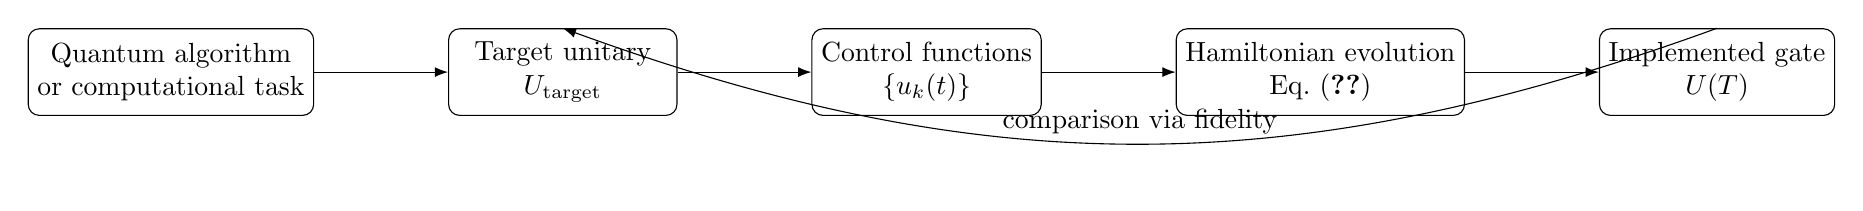
\begin{tikzpicture}[
        >=Latex,
        node distance=1.7cm,
        box/.style={
            draw,
            rounded corners,
            align=center,
            minimum width=2.9cm,
            minimum height=1.1cm
        }
    ]
        \node[box] (alg) {Quantum algorithm\\or computational task};
        \node[box, right=of alg] (target) {Target unitary\\$U_{\mathrm{target}}$};
        \node[box, right=of target] (controls) {Control functions\\$\{u_k(t)\}$};
        \node[box, right=of controls] (dyn) {Hamiltonian evolution\\Eq.~\eqref{eq:time_ordered_propagator}};
        \node[box, right=of dyn] (impl) {Implemented gate\\$U(T)$};

        \draw[->] (alg) -- (target);
        \draw[->] (target) -- (controls);
        \draw[->] (controls) -- (dyn);
        \draw[->] (dyn) -- (impl);
        \draw[->, bend left=20] (impl.north) to node[above]{comparison via fidelity} (target.north);
    \end{tikzpicture}
    \caption{Conceptual pipeline of Hamiltonian-based quantum control. The objective is to determine control functions $\{u_k(t)\}$ that drive the system evolution toward a target unitary gate $U_{\mathrm{target}}$ while satisfying physical and hardware constraints.}
    \label{fig:control_pipeline}
\end{figure}

Once the control problem has been cast in dynamical form, one must define suitable performance metrics. For gate-design applications, the two most important figures of merit are the \emph{accuracy} of the implemented operation and the \emph{time} required to realize it \cite{nielsen2010quantum,niu2018ufo}. In the ideal closed-system setting, a convenient measure of accuracy is the process fidelity between the target unitary and the realized propagator. For a $d$-dimensional computational subspace, one may define
\begin{equation}
F_{\mathrm{pro}}\!\left(U_{\mathrm{target}},U(T)\right)
=
\frac{1}{d^{2}}
\left|
\mathrm{Tr}\!\left(U_{\mathrm{target}}^{\dagger}U(T)\right)
\right|^{2},
\label{eq:process_fidelity}
\end{equation}
with corresponding gate infidelity
\begin{equation}
\mathcal{I}\!\left(U(T),U_{\mathrm{target}}\right)
=
1-F_{\mathrm{pro}}\!\left(U_{\mathrm{target}},U(T)\right).
\label{eq:gate_infidelity_generic}
\end{equation}
For noisy implementations, where the actual evolution is more properly described by a quantum channel $\mathcal{E}$ rather than a unitary operator, the relevant quantity is the average gate fidelity
\begin{equation}
\overline{F}\!\left(\mathcal{E},U_{\mathrm{target}}\right)
=
\int d\psi\,
\bra{\psi}
U_{\mathrm{target}}^{\dagger}
\,\mathcal{E}\!\left(\ket{\psi}\bra{\psi}\right)
U_{\mathrm{target}}
\ket{\psi},
\label{eq:average_gate_fidelity_channel}
\end{equation}
where the integral is taken over pure states with respect to the unitarily invariant Haar measure. In the special case of two unitary operations $U_{\mathrm{target}}$ and $V$, Eq.~\eqref{eq:average_gate_fidelity_channel} reduces to
\begin{equation}
\overline{F}\!\left(U_{\mathrm{target}},V\right)
=
\frac{
\left|\mathrm{Tr}\!\left(U_{\mathrm{target}}^{\dagger}V\right)\right|^{2}+d
}{
d(d+1)
}.
\label{eq:average_gate_fidelity_unitary}
\end{equation}
These expressions are useful because they separate the ideal control objective from the effect of stochastic errors and environmental imperfections. At the same time, gate time $T$ is itself a fundamental performance metric: even a perfectly shaped control sequence becomes less valuable if it is so long that decoherence and drift degrade the computation before completion. For this reason, many quantum-control formulations use a cost functional that balances fidelity against runtime,
\begin{equation}
J[\{u_k\}]
=
\alpha\,\mathcal{I}
+
\beta\,T,
\label{eq:generic_background_cost}
\end{equation}
with positive weights $\alpha,\beta>0$. More realistic formulations then augment Eq.~\eqref{eq:generic_background_cost} by adding penalties for leakage, bandwidth, pulse energy, smoothness, or boundary conditions.

A further conceptual distinction must be made between \emph{gate-based synthesis} and \emph{direct analog control}. In the circuit model of quantum computation, one usually constructs an operation by decomposing it into a sequence of elementary gates drawn from a finite universal set:
\begin{equation}
U_{\mathrm{target}}
\approx
\prod_{\ell=1}^{L} G_{\ell},
\qquad
G_{\ell}\in\mathcal{G},
\label{eq:gate_synthesis_decomposition}
\end{equation}
where $\mathcal{G}$ is a chosen gate alphabet and $L$ is the circuit depth. This paradigm is indispensable in the fault-tolerant setting, where discrete logical gates and error-correction routines play a central role. Nevertheless, at the physical level a quantum processor is still governed by continuous Hamiltonian dynamics, and in near-term devices it is often advantageous to realize a target unitary directly through a single tailored control sequence rather than through a long compiled circuit \cite{niu2018ufo}. Whether this is possible depends on the \emph{controllability} of the driven quantum system. A standard algebraic criterion is formulated in terms of the dynamical Lie algebra
\begin{equation}
\mathfrak{L}
=
\operatorname{Lie}\!\left\{
iH_{0},\,iH_{1},\,\dots,\,iH_{m}
\right\},
\label{eq:dynamic_lie_algebra}
\end{equation}
generated by the drift and control Hamiltonians under repeated commutation \cite{dalessandro2007introduction}. If $\mathfrak{L}=\mathfrak{su}(d)$, or $\mathfrak{u}(d)$ when global phases are retained, then the system is controllable on the $d$-dimensional Hilbert space, meaning that any target unitary can in principle be synthesized through an appropriate choice of controls. This observation is crucial for modern quantum control: it explains why the search for hardware-native, pulse-level implementations can outperform purely discrete decompositions in some regimes, and it also clarifies why practical control design must go beyond abstract universality and confront physical constraints directly. In the remainder of this background chapter, the discussion will therefore move from this general control-theoretic viewpoint to the concrete challenges posed by superconducting circuits, where weak anharmonicity and multilevel structure make the suppression of leakage a central issue.
\end{document}
